% interactcadsample.tex
% v1.03 - April 2017

\documentclass[]{interact}

\usepackage{epstopdf}% To incorporate .eps illustrations using PDFLaTeX, etc.
\usepackage{subfigure}% Support for small, `sub' figures and tables
%\usepackage[nolists,tablesfirst]{endfloat}% To `separate' figures and tables from text if required

\usepackage{natbib}% Citation support using natbib.sty
\bibpunct[, ]{(}{)}{;}{a}{}{,}% Citation support using natbib.sty
\renewcommand\bibfont{\fontsize{10}{12}\selectfont}% Bibliography support using natbib.sty

\theoremstyle{plain}% Theorem-like structures provided by amsthm.sty
\newtheorem{theorem}{Theorem}[section]
\newtheorem{lemma}[theorem]{Lemma}
\newtheorem{corollary}[theorem]{Corollary}
\newtheorem{proposition}[theorem]{Proposition}

\theoremstyle{definition}
\newtheorem{definition}[theorem]{Definition}
\newtheorem{example}[theorem]{Example}

\theoremstyle{remark}
\newtheorem{remark}{Remark}
\newtheorem{notation}{Notation}

\begin{document}

\articletype{ARTICLE DRAFT}

\title{Modelling and optimization of ship's fuel consumption using Random Forest Regression (RFR)}

\author{
\name{Muhammad Fakhruriza Pradana\textsuperscript{a,b}\thanks{Muhammad Fakhruriza Pradana. Email: mfakhruriza@untirta.ac.id}, Hibatul Wafi\textsuperscript{b}, Bernd Noche\textsuperscript{b}}
\affil{\textsuperscript{a}Department of Civil Engineering, University of Sultan Ageng Tirtayasa, Cilegon, Indonesia ; \textsuperscript{b}Institute of Transport Systems and Logistics, University of Duisburg-Essen, Duisburg, Germany}
}

\maketitle

\begin{abstract}
Efforts to model energy-efficient operation of shipping operations using machine-learning methods have emerged due to volatile bunker fuel prices and stringent environmental regulations. It is widely regarded that ship speed is one of the most influential factors impacting ships' fuel oil consumption and as such, accurate modelling of ship speed is paramount to ensure the accuracy of subsequent FOC prediction.\\

This study proposes an intuitive data-driven modelling approach, integrating Automatic Identification System and weather data for modelling of ship states and environmental conditions' impact on FOC. Grey Box Modelling approach divides the speed and FOC prediction into stages, the first stage involves the prediction of speed over ground using Random Forest Regressor. Consequently, the FOC prediction based on predicted speed employs the empirical formula by Holtrop-Mennen, maintaining adherence with established vessel knowledge.\\
  
In the presented case study, optimised SOG prediction achieves $3.94\%$ mean absolute percentage error (MAPE) and $93.41\%$ $R^2$ score. Subsequent FOC prediction from estimated speed yields $86.57\%$ $R^2$ and $12.06\%$ MAPE. The results affirm the proposed approach's viability in predicting energy-efficient ship operations.
\end{abstract}

\begin{keywords}
Energy-efficient operation; Random Forest Regression; Ship speed prediction; Fuel consumption prediction; Grey Box Model; AIS 
\end{keywords}


\section{Introduction}

The marine industry is actively researching efficient ship operation due to rising fuel prices and stricter environmental rules. Fuel costs, known as "bunkers," comprise over 50\% of voyage expenses and up to 75\% of total operating costs, impacting profitability \citep{Bialystocki.2016}. Energy-efficient practices reduce costs and greenhouse gas emissions, crucial with shipping contributing 2.51\% of global emissions \citep{IMO.2020}. This mutual motivation aligns economic benefits with environmental compliance. Stakeholders seek solutions to energy-efficient operation by considering technical and operational approaches. Technical solutions require costly structural and power system alterations \citep{Yan.2021,Li.2022}, prompting interest in the cost-effective, optimisation of operational measures.\\

Significant emphasis is given in this study on optimisation of ship speed due to its substantial impact on fuel consumption which is caused by a third-order non-linear correlation between fuel consumption and ship speed \citep{Wang.2012,Du.2019}. However, the process of optimising the speed prediction model is intricate, appropriate features must be considered as the ship speed is influenced by factors like vessel performance and weather conditions.\\

Fuel consumption models based on historical data and ship parameters lack robustness and sensitivity to noise. To address this, recent research employs data-driven techniques, like machine learning (ML), for ship speed and fuel consumption prediction. ML models showcase strong generalisation capabilities and low prediction errors, although some experts are reluctant to accept the generated models by the machine learning approach due to their complexity, unintuitiveness, and potential violation of vessel physics. The success of data-driven models is also highly dependent on data quality and quantity \citep{Yan.2021,Gkerekos.2019}. Given volatile fuel prices, developing an accurate Fuel Oil Consumption (FOC) prediction model is valuable for maritime stakeholders. This aids in timely economic decisions without violating environmental regulations.\\


\section{Literature Review}\label{sec:literature_review}

\subsection{Modelling Approach for Ship Operation}\label{sec:modelling_type}

\citet{haranen2016white} and \citet{Coraddu.2017} categorised fuel consumption prediction models into three strategies:\\

\textbf{White Box Models (WBM)}: Built on prior mechanistic knowledge and physical principles of a vessel's system, including its structure, design parameters, and propulsion configuration.\\

\textbf{Black Box Models (BBM)}: Data-driven and developed using data from different sailing journeys and historical observations. The Machine Learning (ML) modelling approach focuses on the prediction of bunker consumption at different points in time.\\

\textbf{Grey Box Models (GBM)}: A fusion of WBM and BBM, resulting in a single model that considers both \emph{a priori} knowledge of the vessel and historical sailing data, This method aims to complement the performance of WBM and BBM.\\

Each strategy has strengths and weaknesses. WBM is transparent and comprehensible, rooted in physics and hydrodynamics, but lacks adaptability and generalisation due to its deterministic nature and dependence on prior knowledge. BBM excels in fitting and predicting data but lacks vessel-specific knowledge and can be complex. To achieve good prediction, it requires an abundance of data quantity and good data quality \citep{Halevy.2009}. GBM mitigates these limitations by combining mechanistic understanding with predictive capabilities.\\

The modelling of FOC using GBM requires both components of WBM and BBM. For the BBM modelling part using ML approach, For black-box modelling using ML techniques, it is crucial to have sufficient high-quality data for accurate training \citep{Halevy.2009}. \citet{Yan.2021} categorise the data sources for FOC modelling as follows:
\\

Besides its intended role as a collision avoidance system, Automatic Identification System (AIS) data finds potential in ship behaviour analysis and environmental assessment. The International Maritime Organization (IMO) utilized AIS data to study Greenhouse Gas (GHG) emissions, estimating global shipping emissions \citep{IMO.2020,T.W.P.Smith.2015}. \citet{Rakke.2016} introduced ECAIS as a methodology to compute ship emissions from AIS-derived fuel consumption data using Holtrop-Mennen and literature-based approximations. The study by \citet{Kim.2020b} used AIS data, ship information, and environmental data for estimating Energy Efficiency Operational Indicator (EEOI). The use of AIS data in research aims for data independence, reducing reliance on commercial databases.\\

\subsection{Predictive performance of tree based models}\label{sec:perf_tree_litreview}

Tree-based model is a supervised, highly interpretable BBM modelling approach using machine learning approach which is adept in classification and regression tasks. The model is inherently resistant to multicollinearity problems \citep{Yan.2021}.  Several literature studies reveal its advantages and performance superiority. \citet{Soner.2018} employed ferry data to predict FOC using tree-based models including bagging, random forest (RF), and bootstrap. RF achieved $43.5$ L/h RMSE for fuel consumption, outperforming Artificial Neural Network (ANN) model employed by \citet{Petersen.2012}.\\

\citet{Yan.2020} predicted FOC for a dry bulk ship's voyage using RF. The model incorporated sailing speed, cargo weight, and meteorological conditions, it is able to attain mean absolute percentage error (MAPE) of $7.91\%$ and the RF model outperformed decision tree, ANN, LASSO, and SVR. \citet{Gkerekos.2019} compared ML models to predict daily FOC, RF model achieved $89\%$ and $96\%$ $R^2$ scores with noon data and ADLM system data, respectively. \citet{Li.2022} fused meteorological, voyage, and AIS data to explore the effect of data on ML models for FOC prediction. Tree-based models (bagging and boosting ensembles) including ETR, RFR, AB, GB, XG, and LB were recommended for energy-efficient operation modelling, with RFR particularly displaying the best robustness among the presented ML models in the study. \citet{Abebe.2020} predicted ship speed over ground (SOG) using AIS and weather data. The RF model achieved $98\%$ $R^2$ score and $0.25$ knots RMSE.\\

WBMs for predicting FOC utilize physics and hydrodynamic laws to compute the vessel's resistance, encompassing calm water resistance and additional effects like wind and waves. Then the engine power can be subsequently estimated at a specific speed, facilitating FOC calculation \citep{haranen2016white}. Holtrop-Mennen power estimation method \citet{Holtrop.1984}, is applicable in a wide range \citep{Rakke.2016,Kim.2020b}. \citet{Rakke.2016} utilized AIS data and mechanical information to estimate engine power using Holtrop-Mennen, achieving about $5\%$ model testing error for FOC and GHG emissions estimation. Similarly, \citet{Kim.2020b} estimated Energy Efficiency Operational Index (EEOI) through Holtrop-Mennen-based engine power estimation, enabled by AIS data and weather information.\\

\section{Methodology}\label{sec:big_methodology}

This chapter covers the methodology used to construct the grey box model (GBM). The grey box approach employed in this study is categorised as sequential GBM, which entails a two-stage development process. The initial stage focuses on machine learning modelling using tree-based models. The modelling is carried out using Python in conjunction with \texttt{Scikit-Learn} \citep{FabianPedregosa.2011}. The modelling will use the combination of T-AIS data with weather data from CMEMS and ECMWF. 

\begin{figure}[h]
  \centering
      
\includegraphics[width=.75\textwidth]{00_figures/flowmethod_BBM_alt.png}
      \caption{Scheme of proposed BBM methodology}
      \label{fig:flowchart_BBM}
\end{figure}

The second stage of the modelling process revolves around the power estimation method \citep{Holtrop.1984}. This involves an initial conversion of SOG to STW for estimation of encountered resistance during the voyage, this then facilitates the estimation of the required power i.e. the energy required to propel the ship.

\begin{figure}[h]
  \centering
      
\includegraphics[width=.75\textwidth]{00_figures/flowmethod_WBM.png}
      \caption{Scheme of proposed BBM methodology}
      \label{fig:flowchart_GBM}
\end{figure}

\subsection{Modelling methodologies}\label{sec:tree_model_development}

\subsubsection{Decision Tree (DT) Regressor}\label{sec:dt_theo_j}

The Decision Tree operates by employing nested {\tt if-then} statements based on predefined rules, resulting in a partitioned data space. This process can also be visualized as a binary tree, enhancing interpretability by representing diverse input responses within a single tree \citet{Kuhn.2013, Hastie.2009}.\\

A Decision Tree encompasses distinct nodes: the \textbf{\emph{Root node}} represents the top-level node; \textbf{\emph{Leaf nodes}} (or terminal nodes) yield final prediction outcomes; and \textbf{\emph{Internal nodes}} lie between the root and leaf nodes. The procedure of dividing a node into subsequent nodes is termed \textbf{\emph{splitting}}, where the original node is the \textbf{\emph{parent node}} and the resultant nodes are \textbf{\emph{child nodes}}. In regression tasks, tree growth is often controlled by Mean Square Error (MSE), guided by the Classification and Regression Tree (CART) algorithm, The notation $J(\text{k},\text{t}_k)$ represents the cost function that needs to be minimised.

\begin{equation}\label{eqn:sse}
  \text{MSE}_{\text{s}_i} = \frac{1}{n_{\text{s}_i}}\text{SSE}_{\text{s}_i} \quad \textbf{where} \quad i = (1,2)   
\end{equation}
\begin{equation}\label{eqn:costfun}
  J(\text{k},\text{t}_k) = \frac{1}{n_{\text{s}_1}}\text{SSE}_{\text{s}_1} + \frac{1}{n_{\text{s}_2}}\text{SSE}_{\text{s}_2}
  \begin{cases}
      \text{SSE}_{\text{s}_i} = \sum\limits_{i \in \text{s}_i}(\hat{y}_{\text{s}_i} - y_{\text{s}_i} )^2 \\
      \hat{y}_{\text{s}_i} = \frac{1}{n_{\text{s}_i}}\sum\limits_{i\in \text{s}_i} y
  \end{cases}  
\end{equation}

The process of tree growth stops until either the number of samples for splitting reaches a predefined threshold or when no further split can be found which reduces the MSE. The decisions from optimal splits are visualised through a binary tree representation, enhancing the interpretability and ease of implementation. The inherent logic structure of decision trees enables them to handle diverse data types without extensive preprocessing, including sparse, skewed, continuous, and categorical data. Decision trees also inherently perform feature selection, which is a valuable aspect in modelling \citep{Kuhn.2013}.\\

\begin{figure}
  \label{fig:dtr_tree_trained}
  \centering
  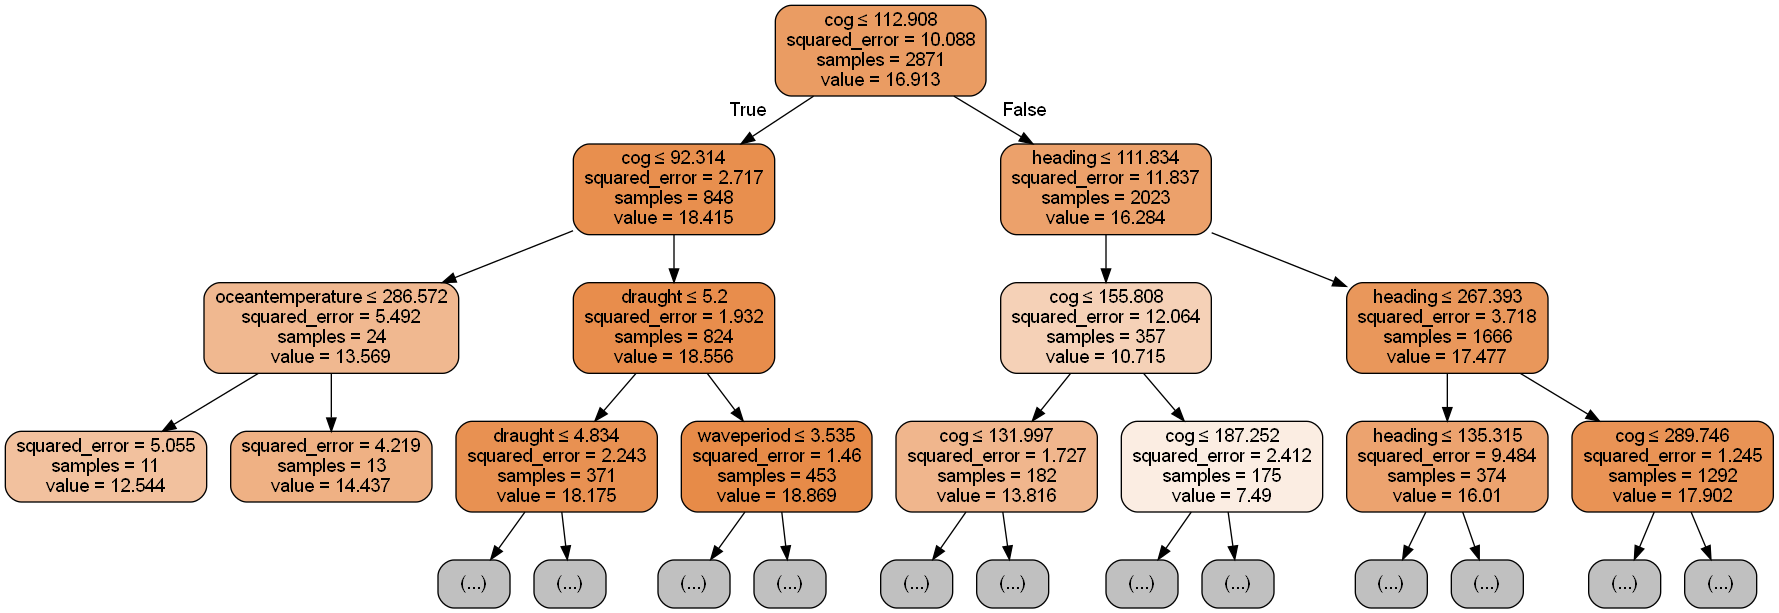
\includegraphics[width=.9\textwidth]{00_figures/dtr_mod_1tree.png}
  \caption{Structure of a Decision Tree (DT) Regressor}
\end{figure}

However, an unconstrained single decision tree is prone to overfitting due to its tendency to closely match the training data. This model's instability can lead to substantial changes in its structure when the data is altered, resulting in a completely different interpretation of splits \citep{Hastie.2009, Kuhn.2013}. To mitigate overfitting, it becomes essential to regularise the decision tree's growth during training. The following parameters control the growth of a single decision tree : 

\begin{itemize}
  \item \texttt{max\_depth}: This hyperparameter is defined as the count of nodes along a path from the root node to its parent node. The default parameter allows full unpruned growth of the tree.
  \item \texttt{min\_samples\_leaf}: This hyperparameter controls the number of samples required to be at the leaf node, where the split point will be considered if the leaf contains at least {\tt min\_samples\_leaf=n} training samples in each left and right branch.
  \item \texttt{min\_samples\_split}: This hyperparameter controls the minimum number of samples i.e. data points required to split a node.    
\end{itemize}

\subsubsection{Random Forest (RF) Regressor}\label{sec:rf_theo_j}

Ensemble learning offers a solution to enhance the performance of Decision Tree (DT) regressors. This concept involves combining the strengths of multiple simpler base models \citep{Hastie.2009}. One prominent ensemble method is the \textbf{\emph{Random Forest}}, introduced by \citet{Breiman.2001}, which involves creating bootstrap samples, randomly selecting splitting features, and aggregating predictions. This approach combines various learning algorithms, referred to as weak learners, with each corresponding to an individual decision tree in the Random Forest. Random forest uses the Bagging (\emph{bootstrap aggregating}) strategy, where it trains each tree using bootstrap samples, where instances from the training set are randomly selected with replacement.\\ 

To further improve bagging, reducing the correlation between trees is applied. This involves introducing randomness during tree construction. Random split selection, as introduced by \citet{Dietterich.2000}, involves selecting a feature from a random subset for each split. This, coupled with the inherent instability of a single decision tree, addresses overfitting and the lack of robustness of DTR. The Random Forest methodology addresses these issues by creating an ensemble of independent, strong learners, resulting in reduced variance and robustness against noisy data \citep{Breiman.2001}. While losing some interpretability compared to basic tree-based models, the impact of each feature in the ensemble can still be quantified \citep{Kuhn.2013}. Random Forest performs better with larger sample sizes, and extensive parameter tuning is often unnecessary for good prediction results \citep{Kuhn.2013, Hastie.2009}.\\

In addition to the hyperparameters used to fine-tune the decision tree, the RF model provides additional hyperparameters to control the growth of the tree:

\begin{itemize}
  \item \texttt{max\_features}: This hyperparameter controls the number of features to be considered when looking for the best split. The default parameter considers all features during training.
  \item \texttt{n\_estimators}: This hyperparameter controls the number of trees i.e. predictors in a forest.
\end{itemize}


\section{Using the \texttt{interact} class file}

For convenience, simply copy the \texttt{interact.cls} file into the same directory as your manuscript files (you do not need to install it in your \TeX\ distribution). In order to use the \texttt{interact} document class, replace the command \verb"\documentclass{article}" at the beginning of your document with the command \verb"\documentclass{interact}".

The following document-class options should \emph{not} be used with the \texttt{interact} class file:
\begin{itemize}
  \item \texttt{10pt}, \texttt{11pt}, \texttt{12pt} -- unavailable;
  \item \texttt{oneside}, \texttt{twoside} -- not necessary, \texttt{oneside} is the default;
  \item \texttt{leqno}, \texttt{titlepage} -- should not be used;
  \item \texttt{twocolumn} -- should not be used (see Subsection~\ref{class});
  \item \texttt{onecolumn} -- not necessary as it is the default style.
\end{itemize}
To prepare a manuscript for a journal that is printed in A4 (two column) format, use the \verb"largeformat" document-class option provided by \texttt{interact.cls}; otherwise the class file produces pages sized for B5 (single column) format by default. The \texttt{geometry} package should not be used to make any further adjustments to the page dimensions.

%If your manuscript has supplementary content you can prepare this using the \verb"suppldata" document-class option, which will suppress the `article history' date. This option must \emph{not} be used on any primary content.


\section{Additional features of the \texttt{interact} class file}

\subsection{Title, authors' names and affiliations, abstracts and article types}

The title should be generated at the beginning of your article using the \verb"\maketitle" command.
In the final version the author name(s) and affiliation(s) must be followed immediately by \verb"\maketitle" as shown below in order for them to be displayed in your PDF document.
To prepare an anonymous version for double-blind peer review, you can put the \verb"\maketitle" between the \verb"\title" and the \verb"\author" in order to hide the author name(s) and affiliation(s) temporarily.
Next you should include the abstract if your article has one, enclosed within an \texttt{abstract} environment.
The \verb"\articletype" command is also provided as an \emph{optional} element which should only be included if your article actually needs it.
For example, the titles for this document begin as follows:
\begin{verbatim}
\articletype{ARTICLE TEMPLATE}

\title{Taylor \& Francis \LaTeX\ template for authors (\textsf{Interact}
layout + Chicago author-date reference style)}

\author{
\name{A.~N. Author\textsuperscript{a}\thanks{CONTACT A.~N. Author.
Email: latex.helpdesk@tandf.co.uk} and John Smith\textsuperscript{b}}
\affil{\textsuperscript{a}Taylor \& Francis, 4 Park Square, Milton
Park, Abingdon, UK; \textsuperscript{b}Institut f\"{u}r Informatik,
Albert-Ludwigs-Universit\"{a}t, Freiburg, Germany} }

\maketitle

\begin{abstract}
This template is for authors who are preparing a manuscript for a
Taylor \& Francis journal using the \LaTeX\ document preparation system
and the \texttt{interact} class file, which is available via selected
journals' home pages on the Taylor \& Francis website.
\end{abstract}
\end{verbatim}

An additional abstract in another language (preceded by a translation of the article title) may be included within the \verb"abstract" environment if required.

A graphical abstract may also be included if required. Within the \verb"abstract" environment you can include the code
\begin{verbatim}
\\\resizebox{25pc}{!}{\includegraphics{abstract.eps}}
\end{verbatim}
where the graphical abstract is to appear, where \verb"abstract.eps" is the name of the file containing the graphic (note that \verb"25pc" is the recommended maximum width, expressed in pica, for the graphical abstract in your manuscript).


\subsection{Abbreviations}

A list of abbreviations may be included if required, enclosed within an \texttt{abbreviations} environment, i.e.\ \verb"\begin{abbreviations}"\ldots\verb"\end{abbreviations}", immediately following the \verb"abstract" environment.


\subsection{Keywords}

A list of keywords may be included if required, enclosed within a \texttt{keywords} environment, i.e.\ \verb"\begin{keywords}"\ldots\verb"\end{keywords}". Additional keywords in other languages (preceded by a translation of the word `keywords') may also be included within the \verb"keywords" environment if required.


\subsection{Subject classification codes}

AMS, JEL or PACS classification codes may be included if required. The \texttt{interact} class file provides an \texttt{amscode} environment, i.e.\ \verb"\begin{amscode}"\ldots\verb"\end{amscode}", a \texttt{jelcode} environment, i.e.\ \verb"\begin{jelcode}"\ldots\verb"\end{jelcode}", and a \texttt{pacscode} environment, i.e.\ \verb"\begin{pacscode}"\ldots\verb"\end{pacscode}" to assist with this.


\subsection{Additional footnotes to the title or authors' names}

The \verb"\thanks" command may be used to create additional footnotes to the title or authors' names if required. Footnote symbols for this purpose should be used in the order
$^\ast$~(coded as \verb"$^\ast$"), $\dagger$~(\verb"$\dagger$"), $\ddagger$~(\verb"$\ddagger$"), $\S$~(\verb"$\S$"), $\P$~(\verb"$\P$"), $\|$~(\verb"$\|$"),
$\dagger\dagger$~(\verb"$\dagger\dagger$"), $\ddagger\ddagger$~(\verb"$\ddagger\ddagger$"), $\S\S$~(\verb"$\S\S$"), $\P\P$~(\verb"$\P\P$").

Note that any \verb"footnote"s to the main text will automatically be assigned the superscript symbols 1, 2, 3, etc. by the class file.\footnote{If preferred, the \texttt{endnotes} package may be used to set the notes at the end of your text, before the bibliography. The symbols will be changed to match the style of the journal if necessary by the typesetter.}


\section{Some guidelines for using the standard features of \LaTeX}

\subsection{Sections}

The \textsf{Interact} layout style allows for five levels of section heading, all of which are provided in the \texttt{interact} class file using the standard \LaTeX\ commands \verb"\section", \verb"\subsection", \verb"\subsubsection", \verb"\paragraph" and \verb"\subparagraph". Numbering will be automatically generated for all these headings by default.


\subsection{Lists}

Numbered lists are produced using the \texttt{enumerate} environment, which will number each list item with arabic numerals by default. For example,
\begin{enumerate}
  \item first item
  \item second item
  \item third item
\end{enumerate}
was produced by
\begin{verbatim}
\begin{enumerate}
  \item first item
  \item second item
  \item third item
\end{enumerate}
\end{verbatim}
Alternative numbering styles can be achieved by inserting an optional argument in square brackets to each \verb"item", e.g.\ \verb"\item[(i)] first item"\, to create a list numbered with roman numerals at level one.

Bulleted lists are produced using the \texttt{itemize} environment. For example,
\begin{itemize}
  \item First bulleted item
  \item Second bulleted item
  \item Third bulleted item
\end{itemize}
was produced by
\begin{verbatim}
\begin{itemize}
  \item First bulleted item
  \item Second bulleted item
  \item Third bulleted item
\end{itemize}
\end{verbatim}


\subsection{Figures}

The \texttt{interact} class file will deal with positioning your figures in the same way as standard \LaTeX. It should not normally be necessary to use the optional \texttt{[htb]} location specifiers of the \texttt{figure} environment in your manuscript; you may, however, find the \verb"[p]" placement option or the \verb"endfloat" package useful if a journal insists on the need to separate figures from the text.

Figure captions appear below the figures themselves, therefore the \verb"\caption" command should appear after the body of the figure. For example, Figure~\ref{sample-figure} with caption and sub-captions is produced using the following commands:
\begin{verbatim}
\begin{figure}
\centering
\subfigure[An example of an individual figure sub-caption.]{%
\resizebox*{5cm}{!}{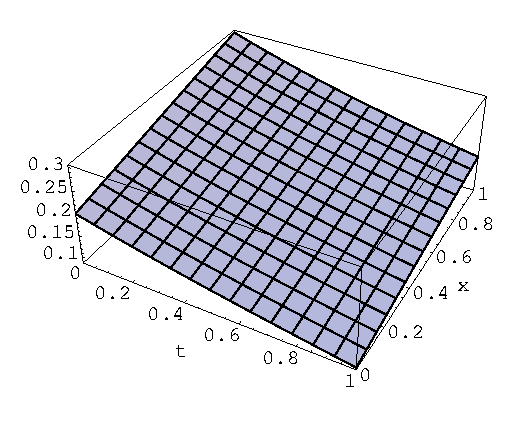
\includegraphics{graph1.eps}}}\hspace{5pt}
\subfigure[A slightly shorter sub-caption.]{%
\resizebox*{5cm}{!}{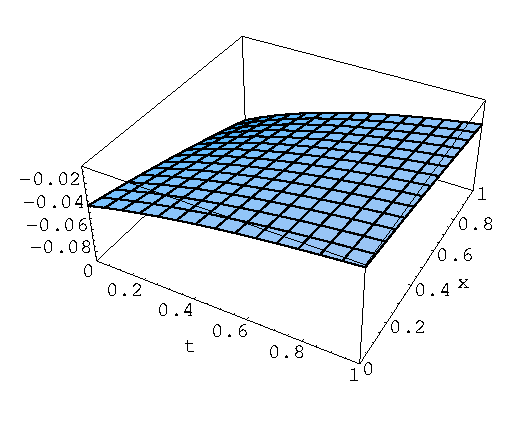
\includegraphics{graph2.eps}}}
\caption{Example of a two-part figure with individual sub-captions
 showing that captions are flush left and justified if greater
 than one line of text.} \label{sample-figure}
\end{figure}
\end{verbatim}
\begin{figure}
\centering
\subfigure[An example of an individual figure sub-caption.]{%
\resizebox*{5cm}{!}{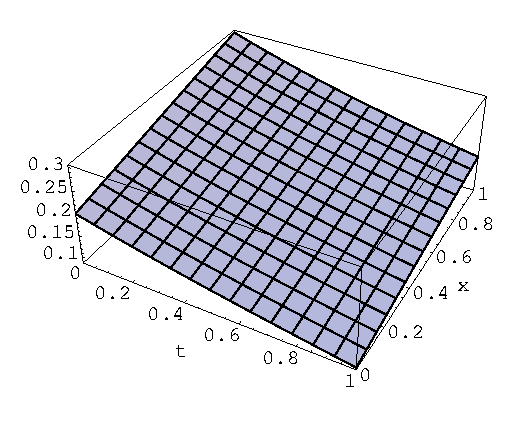
\includegraphics{graph1.eps}}}\hspace{5pt}
\subfigure[A slightly shorter sub-caption.]{%
\resizebox*{5cm}{!}{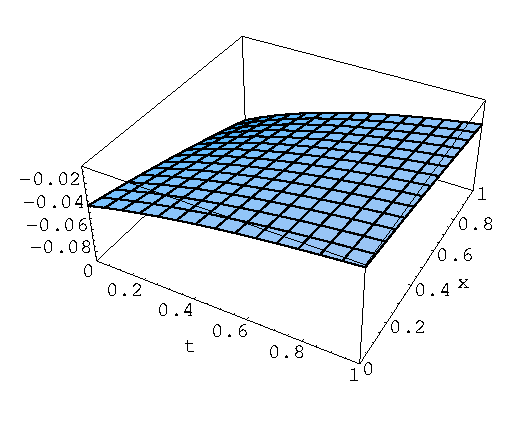
\includegraphics{graph2.eps}}}
\caption{Example of a two-part figure with individual sub-captions
 showing that captions are flush left and justified if greater
 than one line of text.} \label{sample-figure}
\end{figure}

To ensure that figures are correctly numbered automatically, the \verb"\label" command should be included just after the \verb"\caption" command, or in its argument.

The \verb"\subfigure" command requires \verb"subfigure.sty", which is called in the preamble of the \texttt{interacttfssample.tex} file (to allow your choice of an alternative package if preferred) and included in the \textsf{Interact} \LaTeX\ bundle for convenience. Please supply any additional figure macros used with your article in the preamble of your .tex file.

The source files of any figures will be required when the final, revised version of a manuscript is submitted. Authors should ensure that these are suitable (in terms of lettering size, etc.) for the reductions they envisage.

The \texttt{epstopdf} package can be used to incorporate encapsulated PostScript (.eps) illustrations when using PDF\LaTeX, etc. Please provide the original .eps source files rather than the generated PDF images of those illustrations for production purposes.


\subsection{Tables}

The \texttt{interact} class file will deal with positioning your tables in the same way as standard \LaTeX. It should not normally be necessary to use the optional \texttt{[htb]} location specifiers of the \texttt{table} environment in your manuscript; you may, however, find the \verb"[p]" placement option or the \verb"endfloat" package useful if a journal insists on the need to separate tables from the text.

The \texttt{tabular} environment can be used as shown to create tables with single horizontal rules at the head, foot and elsewhere as appropriate. The captions appear above the tables in the \textsf{Interact} style, therefore the \verb"\tbl" command should be used before the body of the table. For example, Table~\ref{sample-table} is produced using the following commands:
\begin{table}
\tbl{Example of a table showing that its caption is as wide as
 the table itself and justified.}
{\begin{tabular}{lcccccc} \toprule
 & \multicolumn{2}{l}{Type} \\ \cmidrule{2-7}
 Class & One & Two & Three & Four & Five & Six \\ \midrule
 Alpha\textsuperscript{a} & A1 & A2 & A3 & A4 & A5 & A6 \\
 Beta & B2 & B2 & B3 & B4 & B5 & B6 \\
 Gamma & C2 & C2 & C3 & C4 & C5 & C6 \\ \bottomrule
\end{tabular}}
\tabnote{\textsuperscript{a}This footnote shows how to include
 footnotes to a table if required.}
\label{sample-table}
\end{table}
\begin{verbatim}
\begin{table}
\tbl{Example of a table showing that its caption is as wide as
 the table itself and justified.}
{\begin{tabular}{lcccccc} \toprule
 & \multicolumn{2}{l}{Type} \\ \cmidrule{2-7}
 Class & One & Two & Three & Four & Five & Six \\ \midrule
 Alpha\textsuperscript{a} & A1 & A2 & A3 & A4 & A5 & A6 \\
 Beta & B2 & B2 & B3 & B4 & B5 & B6 \\
 Gamma & C2 & C2 & C3 & C4 & C5 & C6 \\ \bottomrule
\end{tabular}}
\tabnote{\textsuperscript{a}This footnote shows how to include
 footnotes to a table if required.}
\label{sample-table}
\end{table}
\end{verbatim}

To ensure that tables are correctly numbered automatically, the \verb"\label" command should be included just before \verb"\end{table}".

The \verb"\toprule", \verb"\midrule", \verb"\bottomrule" and \verb"\cmidrule" commands are those used by \verb"booktabs.sty", which is called by the \texttt{interact} class file and included in the \textsf{Interact} \LaTeX\ bundle for convenience. Tables produced using the standard commands of the \texttt{tabular} environment are also compatible with the \texttt{interact} class file.


\subsection{Landscape pages}

If a figure or table is too wide to fit the page it will need to be rotated, along with its caption, through 90$^{\circ}$ anticlockwise. Landscape figures and tables can be produced using the \verb"rotating" package, which is called by the \texttt{interact} class file. The following commands (for example) can be used to produce such pages.
\begin{verbatim}
\setcounter{figure}{1}
\begin{sidewaysfigure}
\centerline{\epsfbox{figname.eps}}
\caption{Example landscape figure caption.}
\label{landfig}
\end{sidewaysfigure}
\end{verbatim}
\begin{verbatim}
\setcounter{table}{1}
\begin{sidewaystable}
 \tbl{Example landscape table caption.}
  {\begin{tabular}{@{}llllcll}
    .
    .
    .
  \end{tabular}}\label{landtab}
\end{sidewaystable}
\end{verbatim}
Before any such float environment, use the \verb"\setcounter" command as above to fix the numbering of the caption (the value of the counter being the number given to the preceding figure or table). Subsequent captions will then be automatically renumbered accordingly. The \verb"\epsfbox" command requires \verb"epsfig.sty", which is called by the \texttt{interact} class file and is also included in the \textsf{Interact} \LaTeX\ bundle for convenience.

Please note that if the \verb"endfloat" package is used, one or both of the commands
\begin{verbatim}
\DeclareDelayedFloatFlavor{sidewaysfigure}{figure}
\DeclareDelayedFloatFlavor{sidewaystable}{table}
\end{verbatim}
will need to be included in the preamble of your .tex file, after the \verb"endfloat" package is loaded, in order to process any landscape figures and/or tables correctly.


\subsection{Theorem-like structures}

A predefined \verb"proof" environment is provided by the \texttt{amsthm} package (which is called by the \texttt{interact} class file), as follows:
\begin{proof}
More recent algorithms for solving the semidefinite programming relaxation are particularly efficient, because they explore the structure of the MAX-CUT problem.
\end{proof}
\noindent This was produced by simply typing:
\begin{verbatim}
\begin{proof}
More recent algorithms for solving the semidefinite programming
relaxation are particularly efficient, because they explore the
structure of the MAX-CUT problem.
\end{proof}
\end{verbatim}
Other theorem-like environments (theorem, definition, remark, etc.) need to be defined as required, e.g.\ using \verb"\newtheorem{theorem}{Theorem}" in the preamble of your .tex file (see the preamble of \verb"interactcadsample.tex" for more examples). You can define the numbering scheme for these structures however suits your article best. Please note that the format of the text in these environments may be changed if necessary to match the style of individual journals by the typesetter during preparation of the proofs.


\subsection{Mathematics}

\subsubsection{Displayed mathematics}

The \texttt{interact} class file will set displayed mathematical formulas centred on the page without equation numbers if you use the \texttt{displaymath} environment or the equivalent \verb"\[...\]" construction. For example, the equation
\[
 \hat{\theta}_{w_i} = \hat{\theta}(s(t,\mathcal{U}_{w_i}))
\]
was typeset using the commands
\begin{verbatim}
\[
 \hat{\theta}_{w_i} = \hat{\theta}(s(t,\mathcal{U}_{w_i}))
\]
\end{verbatim}

For those of your equations that you wish to be automatically numbered sequentially throughout the text for future reference, use the \texttt{equation} environment, e.g.
\begin{equation}
 \hat{\theta}_{w_i} = \hat{\theta}(s(t,\mathcal{U}_{w_i}))
\end{equation}
was typeset using the commands
\begin{verbatim}
\begin{equation}
 \hat{\theta}_{w_i} = \hat{\theta}(s(t,\mathcal{U}_{w_i}))
\end{equation}
\end{verbatim}

Part numbers for sets of equations may be generated using the \texttt{subequations} environment, e.g.
\begin{subequations} \label{subeqnexample}
\begin{equation}
     \varepsilon \rho w_{tt}(s,t) = N[w_{s}(s,t),w_{st}(s,t)]_{s},
     \label{subeqnparta}
\end{equation}
\begin{equation}
     w_{tt}(1,t)+N[w_{s}(1,t),w_{st}(1,t)] = 0,
     \label{subeqnpartb}
\end{equation}
\end{subequations}
which was typeset using the commands
\begin{verbatim}
\begin{subequations} \label{subeqnexample}
\begin{equation}
     \varepsilon \rho w_{tt}(s,t) = N[w_{s}(s,t),w_{st}(s,t)]_{s},
     \label{subeqnparta}
\end{equation}
\begin{equation}
     w_{tt}(1,t)+N[w_{s}(1,t),w_{st}(1,t)] = 0,   \label{subeqnpartb}
\end{equation}
\end{subequations}
\end{verbatim}
This is made possible by the \texttt{amsmath} package, which is called by the class file. If you put a \verb"\label" just after the \verb"\begin{subequations}" command, references can be made to the collection of equations, i.e.\ `(\ref{subeqnexample})' in the example above. Or, as the example also shows, you can label and refer to each equation individually -- i.e.\ `(\ref{subeqnparta})' and `(\ref{subeqnpartb})'.

Displayed mathematics should be given end-of-line punctuation appropriate to the running text sentence of which it forms a part, if required.

\subsubsection{Math fonts}

\paragraph{Superscripts and subscripts}
Superscripts and subscripts will automatically come out in the correct size in a math environment (i.e.\ enclosed within \verb"\(...\)" or \verb"$...$" commands in running text, or within \verb"\[...\]" or the \texttt{equation} environment for displayed equations). Sub/superscripts that are physical variables should be italic, whereas those that are labels should be roman (e.g.\ $C_p$, $T_\mathrm{eff}$). If the subscripts or superscripts need to be other than italic, they must be coded individually.

\paragraph{Upright Greek characters and the upright partial derivative sign}
Upright lowercase Greek characters can be obtained by inserting the letter `u' in the control code for the character, e.g.\ \verb"\umu" and \verb"\upi" produce $\umu$ (used, for example, in the symbol for the unit microns -- $\umu\mathrm{m}$) and $\upi$ (the ratio of the circumference of a circle to its diameter). Similarly, the control code for the upright partial derivative $\upartial$ is \verb"\upartial". Bold lowercase as well as uppercase Greek characters can be obtained by \verb"{\bm \gamma}", for example, which gives ${\bm \gamma}$, and \verb"{\bm \Gamma}", which gives ${\bm \Gamma}$.


\section*{Acknowledgement(s)}

An unnumbered section, e.g.\ \verb"\section*{Acknowledgements}", may be used for thanks, etc.\ if required and included \emph{in the non-anonymous version} before any Notes or References.


\section*{Disclosure statement}

An unnumbered section, e.g.\ \verb"\section*{Disclosure statement}", may be used to declare any potential conflict of interest and included \emph{in the non-anonymous version} before any Notes or References, after any Acknowledgements and before any Funding information.


\section*{Funding}

An unnumbered section, e.g.\ \verb"\section*{Funding}", may be used for grant details, etc.\ if required and included \emph{in the non-anonymous version} before any Notes or References.


\section*{Notes on contributor(s)}

An unnumbered section, e.g.\ \verb"\section*{Notes on contributors}", may be included \emph{in the non-anonymous version} if required. A photograph may be added if requested.


\section*{Nomenclature/Notation}

An unnumbered section, e.g.\ \verb"\section*{Nomenclature}" (or \verb"\section*{Notation}"), may be included if required, before any Notes or References.


\section*{Notes}

An unnumbered `Notes' section may be included before the References (if using the \verb"endnotes" package, use the command \verb"\theendnotes" where the notes are to appear, instead of creating a \verb"\section*").


\section{References}

\subsection{References cited in the text}

References should be cited in Chicago author-date style, e.g.\ `\citep{Alb05,Gre08,Sch87}' or `\ldots~see Smith (1985,~75)'. If there are three authors, list them all in every citation, e.g.\ `\citep{JTL97}'. For more than three authors, cite the first author's name followed by et al. For two or more sources by the same author(s) in the same year, use lower-case letters (a, b, c, ...) with the year to order the entries in the References list and use these letters with the year in the in-text citations, e.g.\ `\citep{FogEHPD04,FogJEE04}'. If two or more authors have the same surname, use their initials with the surnames, e.g.\ `(C.~Doershuk 2010; J.~Doershuk 2009)'. If the first author's names and the years of publication are identical for several references, include enough co-author names to eliminate ambiguity, e.g.\ `(Schonen, Baker, et~al. 2009; Schonen, Brooks, et~al. 2009)'. For further details on this reference style, see the Instructions for Authors on the Taylor \& Francis website.

Each bibliographic entry has a key, which is assigned by the author and is used to refer to that entry in the text. In this document, the key \verb"Fow89" in the citation form \verb"\citep{Fow89}" produces `\citep{Fow89}', and the keys \verb"{Bro86,Bro02,Roh08}" in the citation form \verb"\citep{Bro86,Bro02,Roh08}" produce `\citep{Bro86,Bro02,Roh08}'. The appropriate citation style for different situations can be obtained, for example, by \verb"\citet{Sam06}" for `\citet{Sam06}', \verb"\citealt{Lev05}" for `\citealt{Lev05}', or \verb"\citealp{Mor08}" for `\citealp{Mor08}'. Citation of the year alone may be produced by \verb"\citeyear{Cho08}", i.e.\ `\citeyear{Cho08}', or \verb"\citeyearpar{ChoGul08}", i.e.\ `\citeyearpar{ChoGul08}', or of the author(s) alone by \verb"\citeauthor{Tep05}", i.e.\ `\citeauthor{Tep05}'. Optional notes may be included at the beginning and/or end of a citation by the use of square brackets, e.g.\ \verb"\citep[see][275]{Ell68}" produces `\citep[see][275]{Ell68}'; \verb"\citep[e.g.][]{Wau50}" produces `\citep[e.g.][]{Wau50}'; \verb"\citet[chap.~2]{Str00}" produces `\citet[chap.~2]{Str00}'. A `plain' \verb"\cite" command will produce the same result as a \verb"\citet", i.e.\ \verb"\cite{Wei02}" will produce `\cite{Wei02}'.


\subsection{The list of references}

References should be listed at the end of the main text in alphabetical order by authors' surnames, then chronologically (earliest first).
If references have the same author(s), editor(s), etc., arrange by year of publication, with undated works at the end.
A single-author entry precedes a multi-author entry that begins with the same name.
If the reference list contains two or more items by the same author(s) in the same year, add a, b, etc. and list them alphabetically by title.
Successive entries by two or more authors when only the first author is the same are alphabetized by co-authors' surnames.
If a reference has more than ten named authors, list only the first seven, followed by `et~al.'.
If a reference has no author or editor, order by title; if a date of publication is impossible to find, use `n.d.' in its place.

The following list shows some sample references prepared in the Taylor \& Francis Chicago author-date style.

\bibliographystyle{tfcad}
\bibliography{interactcadsample}

\begin{thebibliography}{}

\bibitem[Albiston(2005)]{Alb05}
Albiston, Catherine~R. 2005. ``Bargaining in the Shadow of Social Institutions:
 Competing Discourses and Social Change in the Workplace Mobilization of Civil
 Rights.'' \emph{Law and Society Review} 39 (1): 11--47.

\bibitem[Brooks and McLennan(2002)]{Bro02}
Brooks, Daniel~R., and Deborah~A. McLennan. 2002. \emph{The Nature of
 Diversity: An Evolutionary Voyage of Discovery}. Chicago: University of
 Chicago Press.

\bibitem[Brooks and Wiley(1986)]{Bro86}
Brooks, Daniel~R., and E.~O. Wiley. 1986. \emph{Evolution as Entropy}. 2nd ed.
 Chicago: University of Chicago Press.

\bibitem[M. Choi(2008)]{Cho08}
Choi, Mihwa. 2008. ``Contesting \emph{Imaginaires} in Death Rituals during the
 Northern Song Dynasty.'' PhD diss., University of Chicago. ProQuest
 (A\,AT\,3300426).

\bibitem[S.~J. Choi and Gulati(2008)]{ChoGul08}
Choi, Stephen~J., and G.~Mitu Gulati. 2008. ``Bias in Judicial Citations: A
 Window into the Behavior of Judges?'' \emph{Journal of Legal Studies} 37
 (January): 87--129.

\bibitem[Ellet(1968)]{Ell68}
Ellet, Elizabeth F.~L. 1968. ``By Rail and Stage to Galena.'' In \emph{Prairie
 State: Impressions of Illinois, 1673--1967, by Travelers and Other Observers},
 edited by Paul~M. Angle, 271--79. Chicago: University of Chicago Press.

\bibitem[Fogel(2004a)]{FogEHPD04}
Fogel, Robert~William. 2004a. \emph{The Escape from Hunger and Premature Death,
 1700--2100: Europe, America, and the Third World}. New York: Cambridge
 University Press.

\bibitem[Fogel(2004b)]{FogJEE04}
Fogel, Robert~William. 2004b. ``Technophysio Evolution and the Measurement of
 Economic Growth.'' \emph{Journal of Evolutionary Economics} 14 (2): 217--21.

\bibitem[Fowler(1989)]{Fow89}
Fowler, Melvin~L. 1989. \emph{The Cahokia Atlas: A Historical Atlas of Cahokia
 Archaeology}. Studies in Illinois Archaeology~6. Springfield: Illinois
 Historic Preservation Agency.

\bibitem[Greenberg(2008)]{Gre08}
Greenberg, Joel, ed. 2008. \emph{Of Prairie, Woods, and Water: Two Centuries
 of Chicago Nature Writing}. Chicago: University of Chicago Press.

\bibitem[Jacobs, Thomas, and Lang(1997)]{JTL97}
Jacobs, Sue-Ellen, Wesley Thomas, and Sabine Lang, eds. 1997. \emph{Two-Spirit
 People: Native American Gender Identity, Sexuality, and Spirituality}. Urbana:
 University of Illinois Press.

\bibitem[Levitt and Dubner(2005)]{Lev05}
Levitt, Steven~D., and Stephen~J. Dubner. 2005. \emph{Freakonomics: A Rogue
 Economist Explores the Hidden Side of Everything}. New York: William Morrow.

\bibitem[Morasse, Guderley, and Dodson(2008)]{Mor08}
Morasse, S{\'e}bastien, Helga Guderley, and Julian~J. Dodson. 2008. ``Paternal
 Reproductive Strategy Influences Metabolic Capacities and Muscle Development
 of Atlantic Salmon (\emph{Salmo salar} L.) Embryos.'' \emph{Physiological and
 Biochemical Zoology} 81 (4): 402--13.

\bibitem[Rohde, Levy, and Kehler(2008)]{Roh08}
Rohde, Hannah, Roger Levy, and Andrew Kehler. 2008. ``Implicit Causality Biases
 Influence Relative Clause Attachment.'' Poster presented at the 21st CUNY
 Conference on Human Sentence Processing, Chapel Hill, NC, March.

\bibitem[Samples(2006)]{Sam06}
Samples, John. 2006. ``The Origins of Modern Campaign Finance Law.'' In
 \emph{The Fallacy of Campaign Finance Reform}, Chap.~7. Chicago: University of
 Chicago Press.

\bibitem[Schuman and Scott(1987)]{Sch87}
Schuman, Howard, and Jacqueline Scott. 1987. ``Problems in the Use of Survey
 Questions to Measure Public Opinion.'' \emph{Science} 236: 957--59.

\bibitem[Strunk and White(2000)]{Str00}
Strunk, William, Jr., and E.~B. White. 2000. \emph{The Elements of Style}.
 4th ed. New York: Allyn and Bacon.

\bibitem[Teplin et~al.(2005)]{Tep05}
Teplin, Linda~A., Gary~M. McClelland, Karen~M. Abram, and Jason~J. Washburn.
 2005. ``Early Violent Death in Delinquent Youth: A Prospective Longitudinal
 Study.'' Paper presented at the Annual Meeting of the American Psychology-Law
 Society, La Jolla, CA, March.

\bibitem[Wauchope(1950)]{Wau50}
Wauchope, Robert. 1950. \emph{A Tentative Sequence of Pre-Classic Ceramics in
 Middle America}. Vol.~1 of \emph{Middle American Research Records}. New
 Orleans, LA: Tulane University.

\bibitem[Weigel and Glazebrook(2002)]{Wei02}
Weigel, Detlef, and Jane Glazebrook. 2002. \emph{\emph{Arabidopsis}: A
 Laboratory Manual}. Cold Spring Harbor, NY: Cold Spring Harbor Laboratory
 Press.

\end{thebibliography}
\bigskip
\noindent This was produced by typing:
\begin{verbatim}
\begin{thebibliography}{}

\bibitem[Albiston(2005)]{Alb05}
Albiston, Catherine~R. 2005. ``Bargaining in the Shadow of Social
 Institutions: Competing Discourses and Social Change in the Workplace
 Mobilization of Civil Rights.'' \emph{Law and Society Review} 39 (1):
 11--47.

\bibitem[Brooks and McLennan(2002)]{Bro02}
Brooks, Daniel~R., and Deborah~A. McLennan. 2002. \emph{The Nature of
 Diversity: An Evolutionary Voyage of Discovery}. Chicago: University
 of Chicago Press.

\bibitem[Brooks and Wiley(1986)]{Bro86}
Brooks, Daniel~R., and E.~O. Wiley. 1986. \emph{Evolution as Entropy}.
 2nd ed. Chicago: University of Chicago Press.

\bibitem[M. Choi(2008)]{Cho08}
Choi, Mihwa. 2008. ``Contesting \emph{Imaginaires} in Death Rituals
 during the Northern Song Dynasty.'' PhD diss., University of Chicago.
 ProQuest (A\,AT\,3300426).

\bibitem[S.~J. Choi and Gulati(2008)]{ChoGul08}
Choi, Stephen~J., and G.~Mitu Gulati. 2008. ``Bias in Judicial
 Citations: A Window into the Behavior of Judges?'' \emph{Journal of
 Legal Studies} 37 (January): 87--129.

\bibitem[Ellet(1968)]{Ell68}
Ellet, Elizabeth F.~L. 1968. ``By Rail and Stage to Galena.'' In
 \emph{Prairie State: Impressions of Illinois, 1673--1967, by Travelers
 and Other Observers}, edited by Paul~M. Angle, 271--79. Chicago:
 University of Chicago Press.

\bibitem[Fogel(2004a)]{FogEHPD04}
Fogel, Robert~William. 2004a. \emph{The Escape from Hunger and
 Premature Death, 1700--2100: Europe, America, and the Third World}.
 New York: Cambridge University Press.

\bibitem[Fogel(2004b)]{FogJEE04}
Fogel, Robert~William. 2004b. ``Technophysio Evolution and the
 Measurement of Economic Growth.'' \emph{Journal of Evolutionary
 Economics} 14 (2): 217--21.

\bibitem[Fowler(1989)]{Fow89}
Fowler, Melvin~L. 1989. \emph{The Cahokia Atlas: A Historical Atlas of
 Cahokia Archaeology}. Studies in Illinois Archaeology~6. Springfield:
 Illinois Historic Preservation Agency.

\bibitem[Greenberg(2008)]{Gre08}
Greenberg, Joel, ed. 2008. \emph{Of Prairie, Woods, and Water: Two
 Centuries of Chicago Nature Writing}. Chicago: University of Chicago
 Press.

\bibitem[Jacobs, Thomas, and Lang(1997)]{JTL97}
Jacobs, Sue-Ellen, Wesley Thomas, and Sabine Lang, eds. 1997.
 \emph{Two-Spirit People: Native American Gender Identity, Sexuality,
 and Spirituality}. Urbana: University of Illinois Press.

\bibitem[Levitt and Dubner(2005)]{Lev05}
Levitt, Steven~D., and Stephen~J. Dubner. 2005. \emph{Freakonomics: A
 Rogue Economist Explores the Hidden Side of Everything}. New York:
 William Morrow.

\bibitem[Morasse, Guderley, and Dodson(2008)]{Mor08}
Morasse, S{\'e}bastien, Helga Guderley, and Julian~J. Dodson. 2008.
 ``Paternal Reproductive Strategy Influences Metabolic Capacities and
 Muscle Development of Atlantic Salmon (\emph{Salmo salar} L.) Embryos.''
 \emph{Physiological and Biochemical Zoology} 81 (4): 402--13.

\bibitem[Rohde, Levy, and Kehler(2008)]{Roh08}
Rohde, Hannah, Roger Levy, and Andrew Kehler. 2008. ``Implicit
 Causality Biases Influence Relative Clause Attachment.'' Poster
 presented at the 21st CUNY Conference on Human Sentence Processing,
 Chapel Hill, NC, March.

\bibitem[Samples(2006)]{Sam06}
Samples, John. 2006. ``The Origins of Modern Campaign Finance Law.'' In
 \emph{The Fallacy of Campaign Finance Reform}, Chap.~7. Chicago:
 University of Chicago Press.

\bibitem[Schuman and Scott(1987)]{Sch87}
Schuman, Howard, and Jacqueline Scott. 1987. ``Problems in the Use of
 Survey Questions to Measure Public Opinion.'' \emph{Science} 236: 957--59.

\bibitem[Strunk and White(2000)]{Str2000}
Strunk, William, Jr., and E.~B. White. 2000. \emph{The Elements of
 Style}. 4th ed. New York: Allyn and Bacon.

\bibitem[Teplin et~al.(2005)]{Tep05}
Teplin, Linda~A., Gary~M. McClelland, Karen~M. Abram, and Jason~J.
 Washburn. 2005. ``Early Violent Death in Delinquent Youth: A
 Prospective Longitudinal Study.'' Paper presented at the Annual
 Meeting of the American Psychology-Law Society, La Jolla, CA, March.
\bibitem[Wauchope(1950)]{Wau50}
Wauchope, Robert. 1950. \emph{A Tentative Sequence of Pre-Classic
 Ceramics in Middle America}. Vol.~1 of \emph{Middle American Research
 Records}. New Orleans, LA: Tulane University.

\bibitem[Weigel and Glazebrook(2002)]{Wei02}
Weigel, Detlef, and Jane Glazebrook. 2002. \emph{\emph{Arabidopsis}:
 A Laboratory Manual}. Cold Spring Harbor, NY: Cold Spring Harbor
 Laboratory Press.

\end{thebibliography}
\end{verbatim}
\bigskip
\noindent Each entry takes the form:
\begin{verbatim}
\bibitem[authors' names(date of publication)]{key}
 Bibliography entry
\end{verbatim}
where `\texttt{authors' names}' is the list of names to appear where the \verb"bibitem" is cited in the text, and `\texttt{key}' is the tag that is to be used as an argument for the \verb"\cite{}" commands in the text of the article. `\texttt{Bibliography entry}' is the material that is to appear in the list of references, suitably formatted. The commands
\begin{verbatim}
\usepackage{natbib}
\bibpunct[, ]{(}{)}{;}{a}{}{,}
\renewcommand\bibfont{\fontsize{10}{12}\selectfont}
\end{verbatim}
need to be included in the preamble of your .tex file in order to generate the citations and bibliography as described above.

Instead of typing the bibliography by hand, you may prefer to create the list of references using a \textsc{Bib}\TeX\ database. The \texttt{tfcad.bst} file needs to be in your working folder or an appropriate directory, and the lines
\begin{verbatim}
\bibliographystyle{tfcad}
\bibliography{interactcadsample}
\end{verbatim}
included where the list of references is to appear, where \texttt{tfcad.bst} is the name of the \textsc{Bib}\TeX\ bibliography style file for Taylor \& Francis' Chicago author-date reference style and \texttt{interactcadsample.bib} is the bibliographic database included with the \textsf{Interact}-CAD \LaTeX\ bundle (to be replaced with the name of your own .bib file). \LaTeX/\textsc{Bib}\TeX\ will extract from your .bib file only those references that are cited in your .tex file and list them in the References section.

Please include a copy of your .bib file and/or the final generated .bbl file among your source files if your .tex file does not contain a reference list in a \texttt{thebibliography} environment.


\section{Appendices}

Any appendices should be placed after the list of references, beginning with the command \verb"\appendix" followed by the command \verb"\section" for each appendix title, e.g.
\begin{verbatim}
\appendix
\section{This is the title of the first appendix}
\section{This is the title of the second appendix}
\end{verbatim}
produces:\medskip

\noindent\textbf{Appendix A. This is the title of the first appendix}\medskip

\noindent\textbf{Appendix B. This is the title of the second appendix}\medskip

\noindent Subsections, equations, figures, tables, etc.\ within appendices will then be automatically numbered as appropriate. Some theorem-like environments may need to have their counters reset manually (e.g.\ if they are not numbered within sections in the main text). You can achieve this by using \verb"\numberwithin{remark}{section}" (for example) just after the \verb"\appendix" command.

Please note that if the \verb"endfloat" package is used on a document containing appendices, the \verb"\processdelayedfloats" command must be included immediately before the \verb"\appendix" command in order to ensure that the floats in the main body of the text are numbered as such.

%\processdelayedfloats %%% See above for an explanation of why this command might be needed.

\appendix

\section{Troubleshooting}

Authors may occasionally encounter problems with the preparation of a manuscript using \LaTeX. The appropriate action to take will depend on the nature of the problem:
\begin{enumerate}
\item[(i)] If the problem is with \LaTeX\ itself, rather than with the actual macros, please consult an appropriate \LaTeXe\ manual for initial advice. If the solution cannot be found, or if you suspect that the problem does lie with the macros, then please contact Taylor \& Francis for assistance (\texttt{latex.helpdesk@tandf.co.uk}).
\item[(ii)] Problems with page make-up (e.g.\ occasional overlong lines of text; figures or tables appearing out of order): please do not try to fix these using `hard' page make-up commands -- the typesetter will deal with such problems. (You may, if you wish, draw attention to particular problems when submitting the final version of your manuscript.)
\item[(iii)] If a required font is not available on your system, allow \TeX\ to substitute the font and specify which font is required in a covering letter accompanying your files.
\end{enumerate}


\section{Obtaining the template and class file}

\subsection{Via the Taylor \& Francis website}

This article template and the \texttt{interact} class file may be obtained via the `Instructions for Authors' pages of selected Taylor \& Francis journals.

Please note that the class file calls up the open-source \LaTeX\ packages booktabs.sty, epsfig.sty and rotating.sty, which will, for convenience, unpack with the downloaded template and class file. The template calls for natbib.sty and subfigure.sty, which are also supplied for convenience.


\subsection{Via e-mail}

This article template, the \texttt{interact} class file and the associated open-source \LaTeX\ packages are also available via e-mail. Requests should be addressed to \texttt{latex.helpdesk@tandf.co.uk}, clearly stating for which journal you require the template and class file.

\end{document}
